\documentclass{isprs}
\usepackage{subfigure}
\usepackage{setspace}
\usepackage{geometry} % added 27-02-2014 Markus Englich
\usepackage{epstopdf}
\usepackage{booktabs}
\usepackage{enumitem}
\usepackage{url}


\geometry{a4paper, top=25mm, left=20mm, right=20mm, bottom=25mm, headsep=10mm, footskip=12mm} % added 27-02-2014 Markus Englich
%\usepackage{enumitem}

%\usepackage{isprs}
%\usepackage[perpage,para,symbol*]{footmisc}

%\renewcommand*{\thefootnote}{\fnsymbol{footnote}}



\begin{document}

\title{Open source approach to urban growth simulation}

\author{
A. Petrasova\textsuperscript{a,b,}\thanks{Corresponding author}\,,
V. Petras\textsuperscript{a,b},
D. Van Berkel\textsuperscript{a},
B. A. Harmon\textsuperscript{a,d},
H. Mitasova\textsuperscript{a,b},
R. K. Meentemeyer\textsuperscript{a,c}
}

\address
{
\textsuperscript{a }Center for Geospatial Analytics, North Carolina State University, USA - dbvanber@ncsu.edu\\
\textsuperscript{b }Department of Marine, Earth, and Atmospheric Sciences, North Carolina State University, USA - (vpetras, akratoc, hmitaso)@ncsu.edu\\
\textsuperscript{c }Department of Forestry and Environmental Resources, North Carolina State University, USA - rkmeente@ncsu.edu\\
\textsuperscript{d }Department of Landscape Architecture, North Carolina State University, USA - baharmon@ncsu.edu\\

}

% \commission{VI, }{VI} %This field is optional.
% \workinggroup{VI/4} %This field is optional.
\icwg{Special Session: SpS 10 - FOSS4G: FOSS4G Session (coorganized with OSGeo)}

\abstract
{
Spatial patterns of land use change due to urbanization and its impact on the landscape
are the subject of ongoing research. Urban growth scenario simulation is a powerful tool
for exploring these impacts and empowering planners to make informed decisions. 
We present FUTURES (FUTure Urban -- Regional Environment Simulation) -- a patch-based,
stochastic, multi-level land change modeling framework as a case showing how
an originally closed and inaccessible model can benefit from integration into open source GIS.
We will describe our motivation for releasing this project as open source
and the advantages of integrating it with GRASS GIS, a free, libre and open source GIS
and research platform for geospatial domain.  
GRASS GIS provides efficient libraries for FUTURES model development
as well as standard GIS tools and graphical user interface for model users.  
Releasing FUTURES as a GRASS GIS add-on simplifies the distribution of FUTURES
across all main operating systems and ensures the maintainability of our project in the future.
We will describe FUTURES integration into GRASS GIS and demonstrate its usage
on a case study in Asheville, North Carolina.
The developed dataset and tutorial for this case study
enable researchers to experiment with the model, explore its potential or even
modify the model for their applications.

% To support adoption of FUTURES, we developed a tutorial and a dataset for Asheville, North Carolina.

% Both tutorial and documentation leverage the existing GRASS GIS infrastructure.

% By providing this simple-to-use model with documentation and the sample dataset,we 

}

\keywords{}

\maketitle

%\saythanks % added 28-02-2014 Markus Englich

\section{INTRODUCTION}\label{INTRODUCTION}

Population growth in cities worldwide drives changes in land use
resulting often in negative impacts on the environment people live in, and
challenging the resilience of local ecosystems.
The need to understand the trade-offs urban planners are facing
gave rise to a number of different land change simulation models,
which proved to be powerful tools to explore
alternative scenarios and their impacts on various aspects of human-environmental systems
\cite{chaudhuri2013sleuth,verburg2002modeling,sohl2007fore,waddell2002urbansim}.
Despite the influence of
spatial structure and connectivity of urbanizing landscape on
biodiversity, water quality, or flood risks \cite{alberti2005effects},
most urban growth models are based on cell-level conversions and 
have not focused on generating realistic spatial structures across scales \cite{jantz2005analysis}.
To bridge the gap between cell- and object-based representation, we developed
FUTURES (FUTure Urban-Regional Environment Simulation), a patch-based, multilevel
modeling framework for simulating the emergence of landscape spatial structure
in urbanizing regions \cite{Meentemeyer2012}.
%
FUTURES model was successfully applied in several cases, for studying land development dynamics in the rapidly
expanding metropolitan region of Charlotte, North Carolina \cite{Meentemeyer2012}, and the analysis of the impacts
of urbanization on natural resources under different conservation strategies \cite{Dorning2015}.
Most recently, FUTURES was coupled with ecosystem services models to examine the impacts of urbanization to several
ecosystem services and their trad-offs in Western North Carolina \cite{Brian2016}.

Since complex human-nature systems cannot be studied in separation anymore,
interdisciplinary researchers have to couple existing simulation models,
where land change modeling plays often a crucial role.
Previous FUTURES applications revealed the potential of the model
to be applied in a wide range of cases with different study systems and aims.
However, the developed model was a prototype not suitable to be shared
with scientific community. Large ``technical depth'' \cite{easterbrook2014open} which
accumulated during model development made it difficult to add new features and run the simulation at larger scales.
In order to continue adding new capabilities to FUTURES and to promote
its usage both inside and outside of land use community,
we decided to revise the FUTURES model implementation
and develop a new version which would be (a) more efficient and scalable, 
(b) as easy to use as possible for wider audience and (c)
fully open source and maintainable in the long run.
To achieve these goals we 
decided that instead of keeping FUTURES as a standalone application,
we would take advantage of existing geospatial software and integrate FUTURES
into open source GRASS GIS \cite{Neteler08}.
By using GRASS GIS' efficient geospatial libraries
we can develop better and higher-level code.
In addition to releasing the
actual code, providing scientific software to community as open
source entails providing documentation, tutorials, installation
instructions, binaries and support, all of which require considerable effort.
By using existing GRASS GIS' infrastructure we could focus on developing the actual materials
instead of managing our own server infrastructure.

In this article we present a new version of FUTURES urban growth model
available as \emph{r.futures} module set from GRASS GIS add-on repository.
New version of FUTURES
streamlines data processing, provides opportunities to study urbanization on megaregion scales,
and allows for more reproducible research in land change community. 
We demonstrate the new version of FUTURES on a case study of 
Asheville metropolitan area in North Carolina, USA.



% Releasing model as open source can be challenging because it does not mean
% just posting source code online, but includes many other tasks, such s









% must be open source to attract users chaudhuri2013sleuth
% experimental prototype
% never meant to be published outside of the lab
% implementovali jsme verzi, ktera funguje
% obratit ty body - pouzili jsme versioning system, ...



% FUTURES model was published in a high impact journal thanks to its scientific 
% merit and novelty and extensive case study validation.
% However, original group of authors have not applied one of the pillars of open science \cite{Rey2014}
% in their research --- sharing the model's source code for other scientists to inspect and
% use for their own research. One of the reasons for not sharing the model
% was the great in difficulties in applying the model
% to new case studies or implementing new functionality.
% The technical problems FUTURES project had to deal with are not new,
% but rather common in scientific community \cite{wilson2014best}:
% \begin{itemize}[noitemsep,nolistsep]
%  \item No versioning system was used, resulting in program
%   full of old, unused, and thus unreadable code.
%   \item Although the model was complicated to configure, little documentation
%   existed and limited number of researchers within the team had the sufficient knowledge to run it.
%   \item Parts of the workflow were not described 
%   \item Parts of the workflow were not automized, increasing the time researchers
%   needed to pre-process data and making the study not reproducible with high probability of making an error.
%   
%   \item Little programming experience in combination with less beginner-friendly
%   language (C++) caused errors and suboptimal model performance.
% \end{itemize}





\section{FUTURES model}
FUTure Urban-Regional Environment Simulation
is a stochastic, patched-based model
for projecting landscape patterns of urban growth \cite{Meentemeyer2012}.
FUTURES has a modular structure consisting of 3 main submodels: DEMAND, POTENTIAL and
PGA (patch-growing algorithm), see Figure \ref{fig:schema}.
Land conversion is driven by projected population demand computed by DEMAND submodel,
and is spatially defined by probability surface derived by POTENTIAL
from multiple environmental and socio-economic predictors.
The population demand and the effects of land change drivers can vary in space by subregions,
such as jurisdictional units, allowing projections across heterogeneous landscape.
FUTURES main strength lies in realistic modeling of the 
spatial structure of urban change by growing
patches parametrized by size and compactness calibrated based on historical data.
For detailed explanation of the FUTURES components, please refer to Meentemeyer et al. (2013).

\begin{figure}[h!]
 \centering
 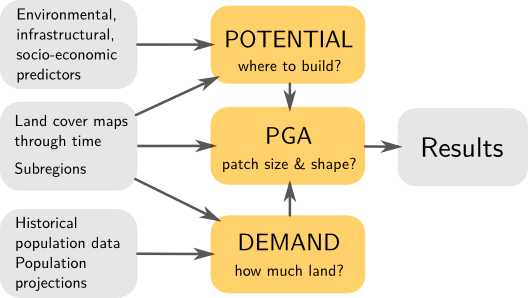
\includegraphics[width=0.9\columnwidth]{./figures/schema.png}
 \caption{Simplified schema of FUTURES conceptual model  with inputs and outputs in gray and submodels in yellow}
 \label{fig:schema}
\end{figure}



% \subsection{Original implementation}
The original implementation of FUTURES consisted mainly of the patch-growing 
algorithm, a standalone program written in a mixture of C and C++.
The PGA program itself utilized inefficient algorithms and required raster data in ASCII
format as input leading to very slow initialization. % such as linear search in a long sorted list.
DEMAND submodel was computed in a spreadsheet and POTENTIAL coefficents
were derived using R statistical software. No official
implementation of these submodels existed so each researcher
developed a different workflow making the verification of their steps
by peers difficult.
%
Several scripts for calibrating patch 
characteristics derived with FRAGSTATS \cite{fragstats} existed, however these tools
were written for one specific case and directory layout of the author,
in too low-level language for that application.
% Data preprocessing required significant amount of time,
% as little automation was done. 
% With little to build upon, we wrote a new implementation of the FUTURES components,
% with the exception of the core PGA program which we improved on significantly.

When revising the original implementation of FUTURES we identified
several issues which needed to be addressed by the new version.
First, it is important to follow best practices for scientific computing \cite{wilson2014best}
including usage of versioning system, writing documentation and testing.
Then we wanted to minimize tasks previously done manually in order to make
them efficient, but also to avoid errors which are often difficult to detect.
When automating the tasks we had to find a compromise between keeping the workflow flexible
and designing it to be simple and efficient.
Further, we focused on making FUTURES scalable for running large scale applications
on a relatively fine spatial resolution.
Finally, we designed FUTURES to be more user-friendly and easy to test so that
anyone can confidently apply it for their research.



\section{INTEGRATION IN GRASS GIS}
GRASS GIS has had a long history as a platform for scientific models \cite{chemin2015grass}.
As an open source GIS used by researchers worldwide and one of the founding projects of OSGeo,
GRASS GIS provides a stable environment for the development of
scientific models studying problems from various domains
including geomorphology, hydrology, planetary science, landscape ecology, hazard mapping, archaeology, renewable energy 
or transportation.
Thanks to the numerous scientist and developers, GRASS GIS today provides a large spectrum of geospatial modules
ranging from basic GIS functionality to highly specialized models.
Most of the specialized tools are not part of standard GRASS GIS installation
but are easily accessible from add-on repository.

Our decision to integrate FUTURES into GRASS GIS as an add-on is
based on several reasons, where some are specific to FUTURES but others would be applicable to any
spatial scientific model.
First, integration into GIS equips both users and developers
with many standard geospatial tools which simplify implementation of a model,
and streamlines pre- and post-processing and visualization.
From the point of view of the model developer, GRASS provides
raster library for highly efficient data reading and writing.
FUTURES therefore does not have to read in ASCII files anymore,
significantly reducing time needed for initialization.
Furthermore, raster data from FUTURES simulation are efficiently compressed.
Despite ever increasing disk space, it is still quite important to reduce the file size, especially for
stochastic spatio-temporal simulations which are typically generating huge datasets.
To achieve best speed performance,
most GRASS GIS functionality is implemented in C.
We could therefore take advantage of the fact that FUTURES was originally written
in a mixture of C and C++ and proceed with the code integration without major rewriting.
For portability reasons we later decided to use C99 standard.
Beside C and C++ as the preferred languages for computationally expensive algorithms,
GRASS GIS supports Python as the main scripting language. This is crucial
for many FUTURES data preparation steps which need to be automated.
Both users and developer can appreciate GRASS' automatic generation of
command line, Python and graphical use interfaces (GUI).
By one simple definition of module options in C or Python modules
we can call the same module from a GUI dialog, a Python or Bash script.
Having a graphical interface is crucial to make FUTURES easy to use,
especially for users on Windows platform. However, for more advanced applications
where FUTURES would run in parallel on a high performance computer,
we need Python or Bash interface.
GRASS GIS provides infrastructure for publishing and distribution of
models to users on all major platforms.
Models and tools in GRASS GIS Add-on repository\footnote{\url{https://grass.osgeo.org/download/addons/}}
can be easily browsed and installed including their documentation,
which relieves researchers willing to share their models of the burden of maintaining necessary infrastructure.




\subsection{Implementation}
We implemented FUTURES as a set of GRASS GIS modules starting with a common prefix \emph{r.futures}:
\begin{itemize}[noitemsep,nolistsep]
 \item \emph{r.futures.demand} extrapolates area of developed land from population trends and projections,
 \item \emph{r.futures.devpressure} computes development pressure predictor,
 \item \emph{r.futures.potential} models the development probability surface through multi level logistic regression,
 \item \emph{r.futures.calib} calibrates patch sizes and shapes,
 \item \emph{r.futures.pga} simulates urban development using patch growing algorithm.
\end{itemize}
In addition, we implemented add-on \emph{r.sample.category} needed for the workflow, but
since its functionality is not specific to FUTURES, we kept it separate.
All these add-ons can be conveniently installed from GRASS GIS from GUI or command line%
\footnote{\texttt{g.extension r.futures}}. 
Each individual add-on has its manual page accessible both online and offline.
Figure \ref{fig:schemaGRASS} shows FUTURES workflow and inputs needed for each tool.
In the following sections we describe the developed tools, their functionality and implementation in GRASS GIS.


\begin{figure}[h!]
 \centering
 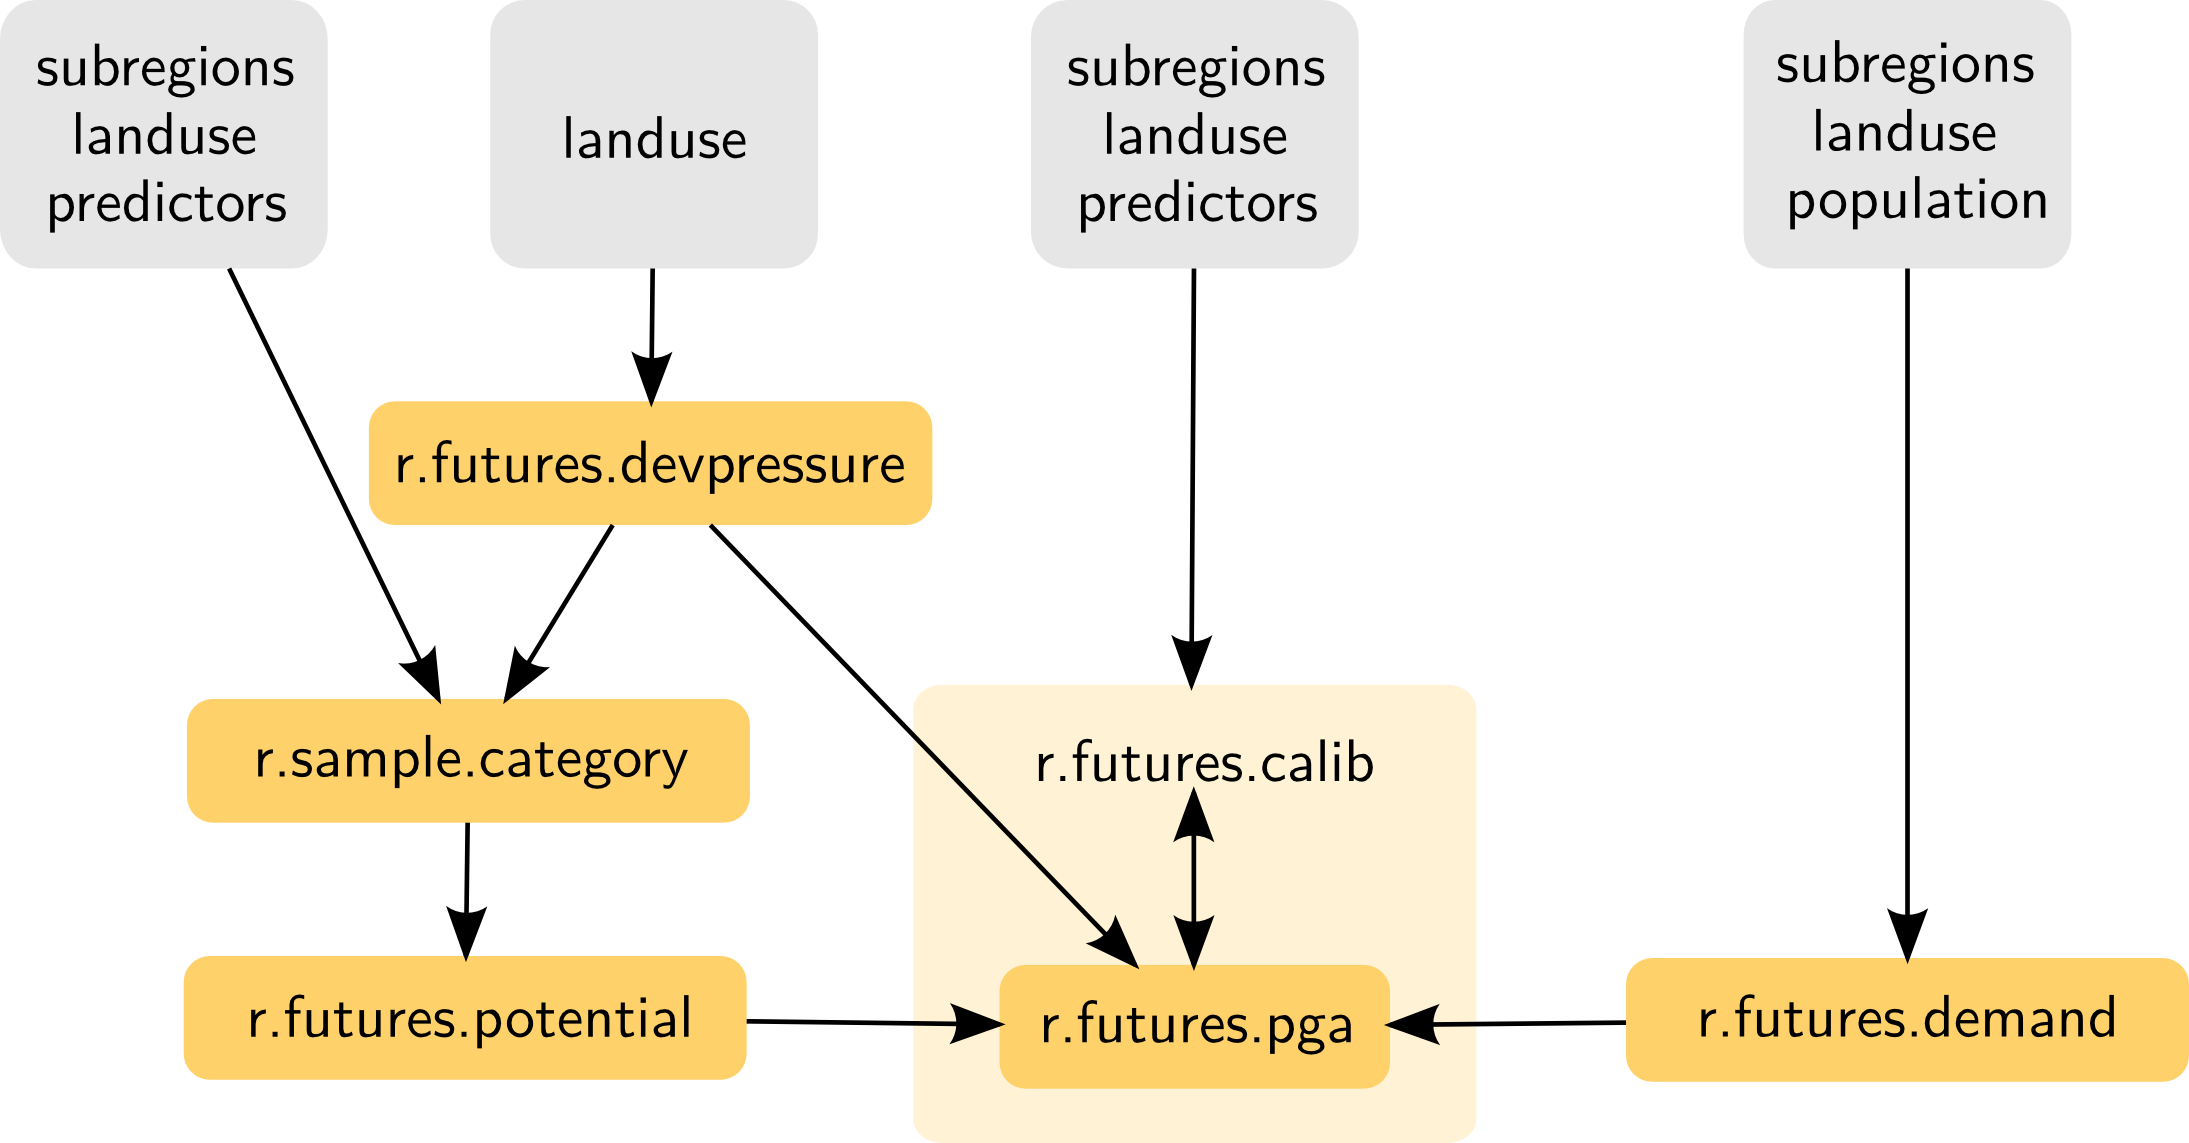
\includegraphics[width=\columnwidth]{./figures/grass_futures_diagram.png}
 \caption{Diagram of FUTURES workflow showing how are \emph{r.futures} modules (yellow boxes) chained 
 and what are their input data (grey boxes). As indicated by the light yellow box,
 module \emph{r.futures.calib} calls \emph{r.futures.pga}.}
 \label{fig:schemaGRASS}
\end{figure}


\subsubsection{r.futures.demand}
Based on historical land development and population growth, DEMAND submodel 
(implemented in \emph{r.futures.demand})
projects the rate of per capita land consumption for each year of the simulation
and each subregion. This Python module uses GRASS GIS Python Scripting
Library and libraries NumPy, SciPy and matplotlib for scientific computing
to approximate the relation between population and land consumption
by a statistical model described by linear, logarithmic or exponential curve.
For example, logarithmic relation means that growing population requires
less developed land per person over time.
Having enough data points, the module
can select best curve for each subregion based on residuals.
The main output is a plain text files with tab-separated values
representing the number of cells to be converted to developed land each year for each subregion.
To allow visual inspection of the results, the module
plots the resulting curves and projected points for each subregion (Figure \ref{fig:demand}).
Module \emph{r.futures.demand} provides a fast way to estimate
the land demand for a large number of subregions with diverse population
trends and allows us to quickly explore different population scenarios.

\begin{figure}[h!]
 \centering
 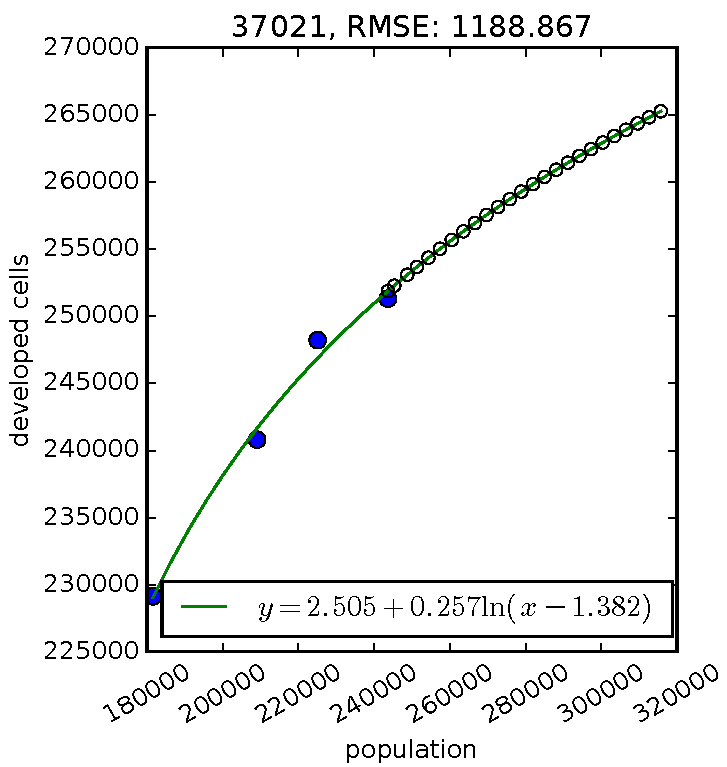
\includegraphics[width=0.4\textwidth]{./figures/plot_demand.pdf}
 \caption{Example of \emph{r.futures.demand} output plot showing
 the logarithmic relation between population and land consumption
 for county with ID 37021.
 Observed data are showed as blue dots, predicted data as circles.
 }
 \label{fig:demand}
\end{figure}

\subsubsection{r.futures.devpressure}
Development pressure is one of the most
important predictors of where
the development is likely to happen
and for each cell it is computed as a distance decay function of neighboring
developed cells \cite{Meentemeyer2012}.
Comparing to a tool previously used for computing the development pressure,
the new Python module \emph{r.futures.devpressure} provides a faster and more efficient 
implementation by taking advantage of the existing GRASS GIS 
module \emph{r.mfilter} written in C for moving window analysis with custom designed matrix filters.
By precomputing the matrix of distances we avoid repeated distance computations
resulting in faster processing. Moreover, the new implementation
minimizes the required memory and can be therefore used for
large regions where the previous tool failed.

\subsubsection{r.futures.potential}
uses multilevel logistic regression  to model the development
suitability based on environmental, infrastructural, and socio-economic predictors such as distance to roads.
We randomly sample these predictors and the observed change from undeveloped to developed cells
to estimate the coefficients of the multilevel logistic regression.
The core of this
module is a script in R language \cite{rstats} which uses package lme4 \cite{lme4}
for fitting generalized linear mixed-effects models and package MuMIn \cite{mumin}
for automatic model selection.
The output file is a plain text file with tab-separated regression coefficients.
% to assist with the selection of the most suitable model.
This script is wrapped in Python for more seamless processing
and chaining of the modules. 
The coupling between R, Python and GRASS GIS
is intentionally very loose to make the workflow possible in the Windows environment
where some of the other, more elegant, options such as
rpy2\footnote{Python package for using R from Python \url{http://rpy2.bitbucket.org/}} are complicated to use.
We use GRASS GIS add-on \emph{r.sample.category} for stratified sampling of the observed new development and predictors.
Although we developed this add-on for urban growth modeling with FUTURES,
its application is much broader and therefore we decided not to include
it in the \emph{r.futures} tool set, but rather keep it general to encourage its usage
in other applications.


\subsubsection{r.futures.pga}
as the main engine of FUTURES simulates urban growth using inputs from
DEMAND and POTENTIAL submodels.
% modules r.futures.demand and r.futures.potential. 
The patch growing algorithm (PGA) stochastically allocates
a seed for new development across the development suitability surface,
challenges it by comparing to a random number between 0 and 1, and
if it survives, a discrete patch is grown \cite{Meentemeyer2012}. This process repeats
until the number of converted cells specified by DEMAND is met.
Then based on the newly developed cells, development pressure predictor and subsequently
the development suitability values are updated.
(the development suitability is computed only internally
from predictors and regression coefficients supplied by POTENTIAL).
We kept the original patch growing algorithm,
however we significantly improved its implementation to make it
faster, more memory efficient and simpler to use.
We replaced a custom, undocumented configuration file with a standard module interface
usable from GUI or command line, and restructured the input and output
parameters and their names to be easy to understand for users.
We used efficient GRASS GIS libraries for reading and writing of raster data
which minimized the time needed for simulation initialization.
Instead of reading ASCII files, FUTURES now reads raster in GRASS native format,
which decreased the time needed for model initialization from several minutes to several seconds
for a region with tens of millions of cells.
Further, we replaced static allocation of internal structures with dynamic allocation
and reduced the overall memory requirements to
enable running FUTURES on large regions with tens or hundreds of counties
as well as smaller areas such as the area of our case study.
Finally, by using appropriate programming techniques, we increased the
speed of the algorithm significantly.


\subsubsection{r.futures.calib}
We developed a dedicated Python module for calibration of patch sizes and shapes
which runs the simulation, specifically module \emph{r.futures.pga},
with different combinations of patch parameters and outputs a table
with scores for each combination of patch parameters. Simulation for each combination is repeated
multiple times to account for the stochasticity of the model.
To speed up the calibration process, \emph{r.futures.calib} can take advantage of multiple
computer cores.

\section{CASE STUDY}
To demonstrate how the new FUTURES framework
can be used for urban growth simulation,
we present here a case study of 
Asheville metropolitan area located in Blue Ridge Mountains in the west of North Carolina, USA.
The region consists of five counties with total area of 6,271 km$^2$ and around 477,000 people
based on 2014 population estimates,
and is characterized by rapid population growth around Asheville, the largest city of the region.
New development is constrained by the steep mountain terrain and large national and state parks.
We simulate urban growth from 2012 to 2030 using publicly available data,
including National Land Cover Database  \cite{nlcd2011,nlcd2006,nlcd2001,nlcdretro},
county population past estimates and future projections \cite{NCOSBM},
boundaries and roads provided by United States Census Bureau's database (TIGER)
and digital elevation model from National Elevation Dataset (NED) distributed by USGS.

\begin{figure}[h!]
 \centering
 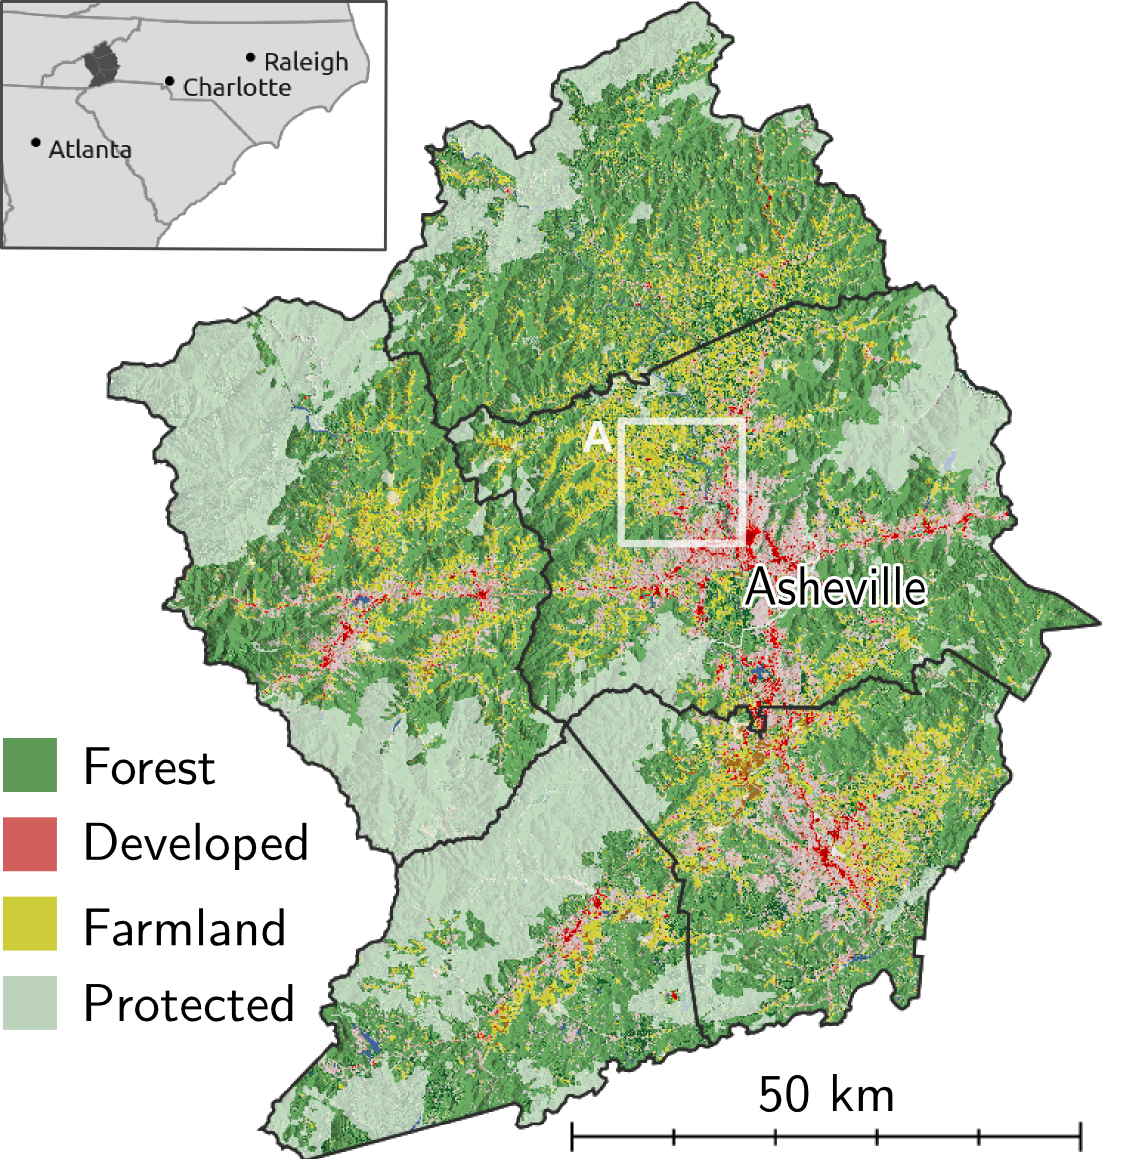
\includegraphics[width=\columnwidth]{./figures/study_area_all.png}
 \caption{2011 land cover \protect\cite{nlcd2011} and protected areas \protect\cite{anderson2011conservation} in Asheville metropolitan area
 in west part of North Carolina, USA. Inset A is used in Figure \ref{fig:results}.}
 \label{fig:study_area}
\end{figure}

\subsection{Approach}
FUTURES simulation consists of several steps, namely
(a) data preprocessing,
(b) estimating of per capita land consumption controlling the total area of converted land,
(c) deriving the development suitability statistical model to control where the new development happens,
(d) calibrating patch size and shape and finally (e) running the urban growth simulation.

\subsubsection{Data preparation}
The core input data for urban growth modeling with FUTURES is a timeseries of land cover maps,
which can be derived by various methods from satellite imagery. In this study
we use National Land Cover Database (NLCD) product by USGS for years 2001, 2006 and 2011
and 1992/2001 Retro\-fit Land Cover Change Product to derive a 30-meter binary representation
of developed areas. We exclude from further analysis areas of national and state parks,
water bodies and wetlands. By using NLCD product available for the entire USA we
allow for easier reproducibility and application of the workflow for other study areas.
We obtained population statistics from North Carolina Office of State Budget and Management,
which are based on 2000 and 2010 census and include past as well as future estimates
of population per county for each year up to 2035. Data for 5 studied counties
were extracted and formated as a comma-separated values (CSV) file.

\subsubsection{DEMAND}
From the series of binary rasters of developed areas and
population statistics we derived the relation between population
and land consumption to model how much land will be developed
each year of the simulation.
Using module \emph{r.futures.demand} we explored different curve fitting
methods and derived the per capita land consumption
from period 1992 to 2011 characterized by
% similar increase in population as in 1992 to 2001 period but significantly
growing population with decreasing demand for land per person over time.
We expect similarly low rates of per capita land consumption
in the following years due to the development restricted by mountainous terrain and
large protected areas.
Based on RMSE and visual inspection of the plots
created by \emph{r.futures.demand} we
selected either linear or logarithmic relation % ($y = a \ln(x) + c$)
for each county, where the function coefficients are found automatically
using linear regression implemented in \emph{r.futures.demand} (Figure \ref{fig:demand}).

\subsubsection{POTENTIAL}
We used multilevel logistic regression to predict
where the new development happens based on
environmental, infrastructural, and socio-economic site suitability
predictors. 
Using \emph{r.sample.category} we sampled predictors on 8000 
randomly selected locations and estimated the model coefficients
using R package lme4 integrated into module \emph{r.futures.potential}.
The sample points were stratified by the response variable
where newly developed sites since 1992 have value 1
and undeveloped sites in 2011 have value 0.
We included counties as the group level indicator
in the multilevel model to account for differences
across jurisdictional boundaries.
From the initial list of hypothesized predictors
(slope, distance to water, protected areas, interchages,
travel time to cities and towns, forest occurrence and road density)
we identified a set of predictors (Table \ref{tab:predictors})
resulting in a model with lowest AIC (Akaike information criterion) score.
By repeating random sampling and model selection multiple times
we verified the robustness of the selected predictors.
Beside the already  mentioned predictors, we included also development pressure,
 a special, dynamic predictor which is being
 updated during the simulation based on new simulated development
 and thus allows for positive feedback.
We computed the initial development pressure raster
with \emph{r.futures.devpressure}, its subsequent updates
are performed in memory during the simulation.
and statistical model selection.

\begin{table}[htp]
 \centering
\begin{center}
\begin{tabular}{lrr}
\toprule
Predictors & Estimate{\scriptsize *} & Std. Error \\ \midrule
Intercept (varies by county) & -0.807 & 0.169\\
Development pressure & 0.031 & 0.005\\
Road density & 0.109 & 0.006\\
Forest occurrence& -0.031& 0.001 \\
Distance to protected areas & -0.115 & 0.028\\
\bottomrule
{\scriptsize * all P-values $<$ 0.001}
\end{tabular}
\end{center}
 \caption{List of selected predictors and estimated coefficients
 for site suitability model}
 \label{tab:predictors}
\end{table}

\subsubsection{Patch calibration}
Prior to running the urban growth simulation implemented in \emph{r.futures.pga}
we calibrated the input patch compactness and size to match
the simulated patterns to the observed patterns from period from 1992 to 2011.
Since calibration is a time consuming process, we ran module
\emph{r.futures.calib} only for Buncombe county with Asheville city
where most new development occurs and applied the results to the rest of our study region.
For each combination of patch parameters we compared the patch characteristics 
averaged from 20 runs of the urban growth simulation with the known patches.
Based on the score we selected patch parameters resulting in high compactness
which is expected for mountainous regions.

\begin{figure*}[t]
 \centering
 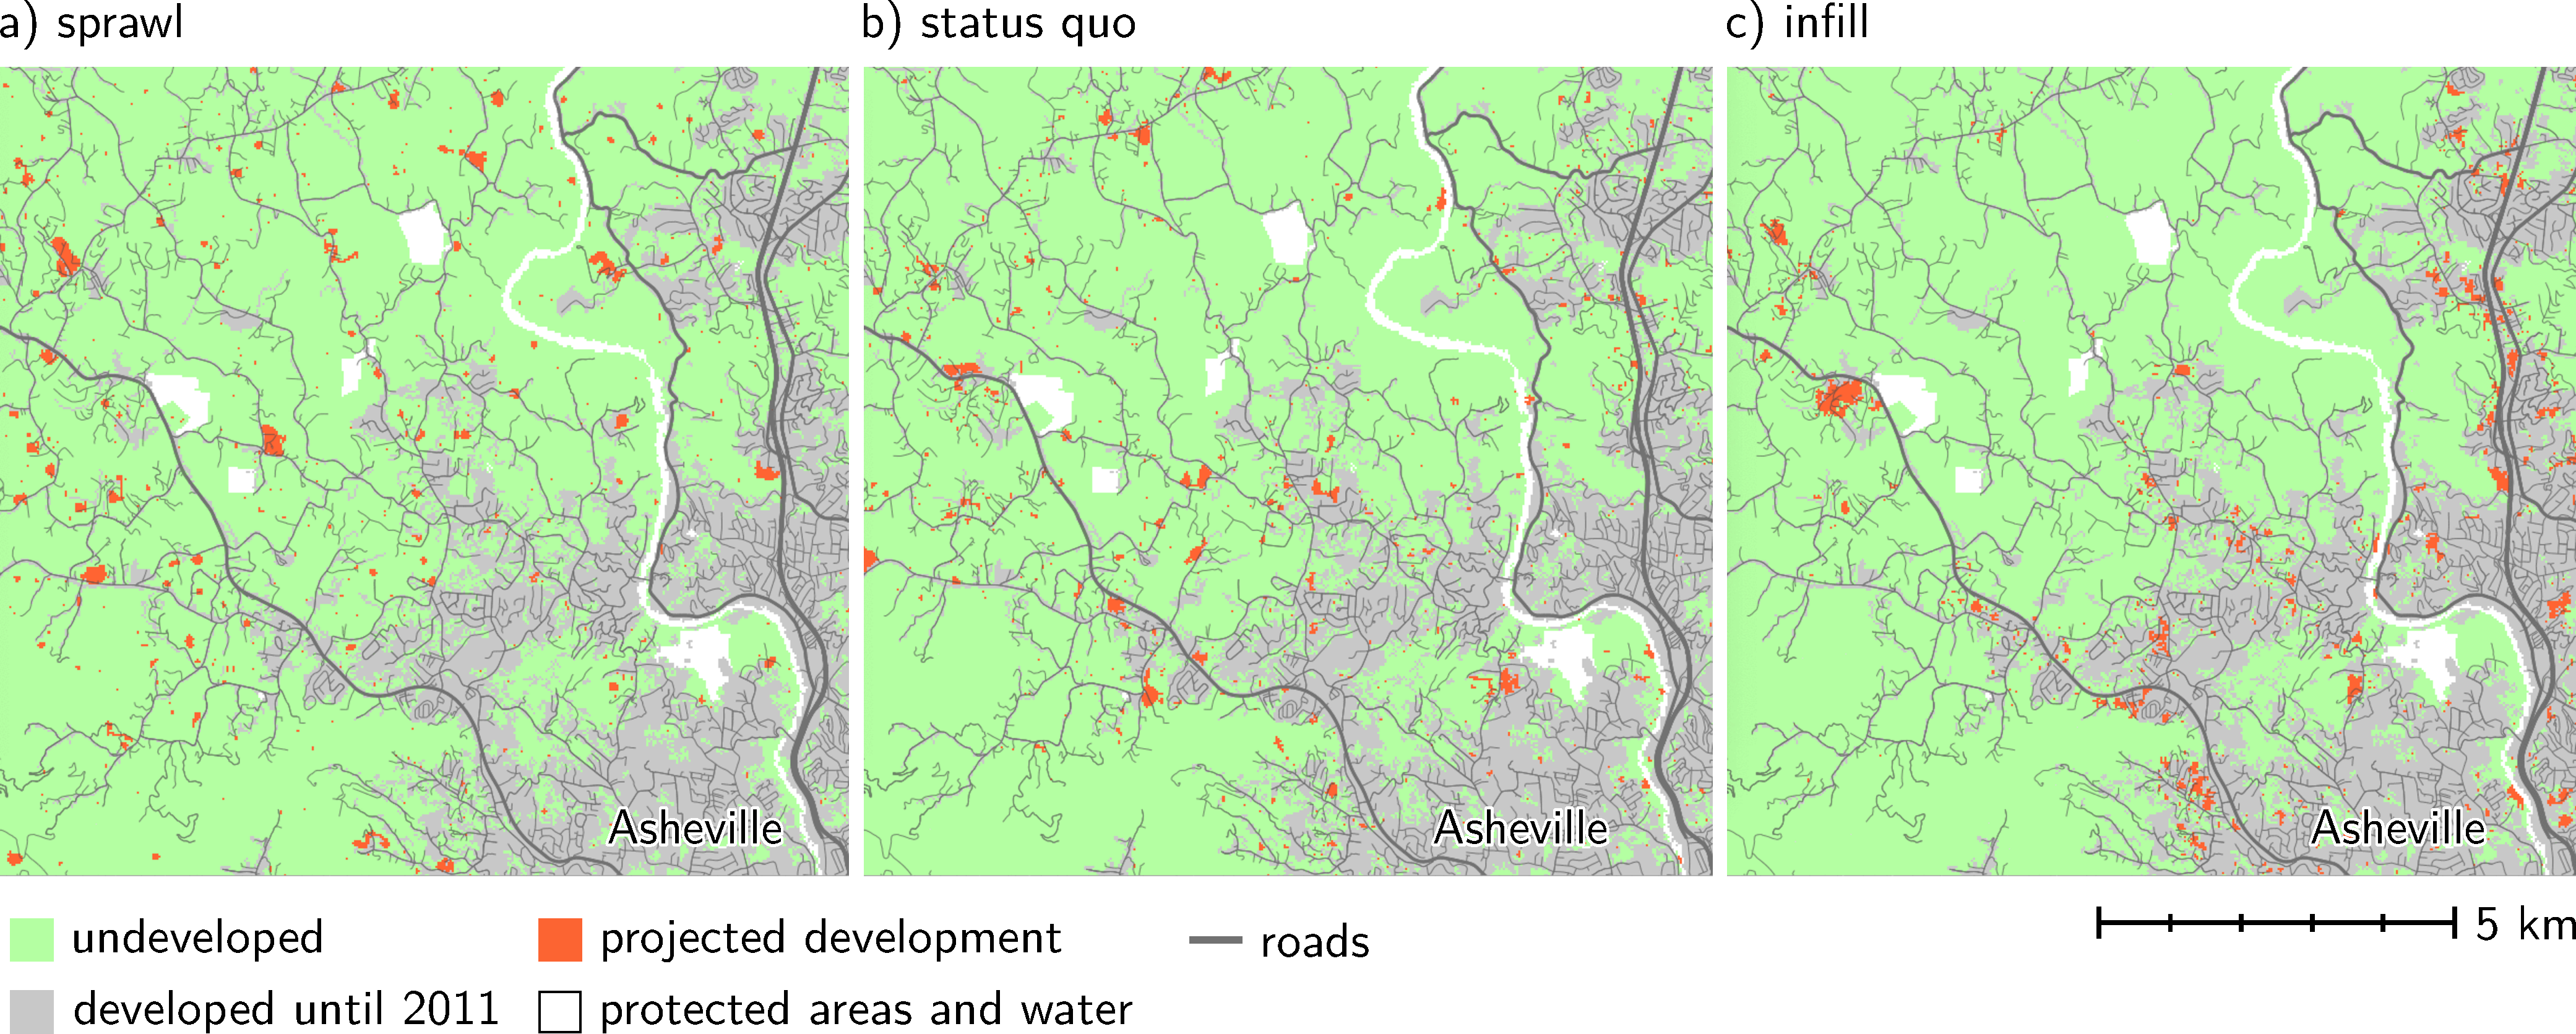
\includegraphics[width=2.0\columnwidth]{./figures/results_maps.pdf}
 \caption{Results of three realizations of multiple stochastic runs with different scenarios.
 Depending on the scenario, simulated development is more diffuse (a) or more compact (c).}
 \label{fig:results}
\end{figure*}

\subsubsection{Urban growth simulation}
Having collected all necessary input data, we ran 
\emph{r.futures.pga} with 1 year step until 2035 for the entire study region at 30 m resolution.
To account for different future policies regarding new development, we explored
scenarios altering the site suitability to encourage infill or sprawl by changing
incentive\_power parameter of \emph{r.futures.pga}. This values transforms
the probability $p$ a cell is developed to $p^x$ where $x = 1$ represents status quo,
higher values of $x$ result in infill and lower values in sprawl.
Beside status quo we simulated additional scenarios with $x$ equals 0.25, 0.5, 2 and 4.
We repeated each scenario 50 times to account for the model's stochastic behavior.



\subsection{Results}
The resulting development patterns of three realizations of the random runs
are visible in Figure \ref{fig:results}
for status quo, infill ($x = 4$) and sprawl ($x=0.25$).
The simulated patches realistically mimic the current patches of development in shape and size
and are mostly but not exclusively adjacent to roads as expected.
% Such fidelity is important to 
Further, we post-processed the results to look at how different urban growth policies
influence the loss of forest and agriculture land in the Asheville area
(Figure \ref{fig:results_plot})
by averaging the loss of both land use categories over the 50 runs.
In all scenarios, forest is affected by future development more than farmland
with extreme case of urban sprawl which results in twice as much developed forest area than farmland.
Status quo shows the smallest difference between the converted area of the two categories
and infill scenario impacts slightly more forest area, possibly because 
developed areas are largely surrounded by forest patches.
% Further analysis could explore the effects of future development on
% forest fragmentation or landscape connectivity.


\begin{figure}
 \centering
 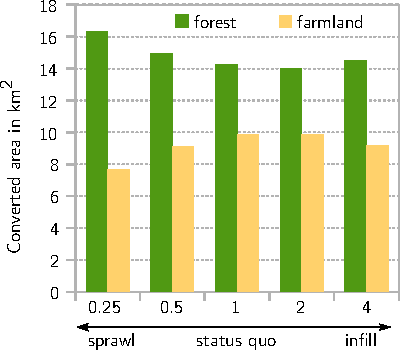
\includegraphics[width=0.9\columnwidth]{./figures/converted_land.pdf}
 \caption{Area in km$^2$ of converted land from forest (green) and farmland (yellow) to urban
 differs for urban sprawl and infill scenarios. Numbers $0.25$ to $4$ represent the exponent $x$ which
 transforms development probability $p$ to $p^x$.}
 \label{fig:results_plot}
\end{figure}

Table \ref{tab:benchmark} shows the computational resources
necessary for running this case study and compares 
the time and memory requirements with the original
implementation of FUTURES. Note that
our study area is fairly small (12 million cells)
and when applied to larger regions with more projected development, 
the expected speed gain is even more significant
as we changed the complexity of one of the core algorithms from linear to logarithmic.
Thanks to the individual stochastic runs being independent on one another
the simulation belongs to the category of 
``embarrassingly parallel''  problems \cite{herlihy2012art}
requiring little effort to distribute the computation on multiple computer cores.

The input data and instructions to run the model are available as part of material
developed for US-IALE 2016 Annual Meeting workshop on FUTURES\footnote{\url{https://grasswiki.osgeo.org/wiki/Workshop_on_urban_growth_modeling_with_FUTURES}}.

\begin{table}[htp]
 \centering
\begin{center}
\begin{tabular}{lccc}
\toprule
FUTURES version & memory & 1 run & all runs (250)\\ \midrule
original & 1.7 GB & 60 s & 4 h 10 min\\
r.futures  & 0.86 GB & 19 s & 1 h 20 min\\
\bottomrule
\end{tabular}
\end{center}
 \caption{Time and memory needed to run the simulations
 with old FUTURES version and with the new \emph{r.futures}
 implemented in GRASS GIS on a laptop with 64-bit Ubuntu 14.04 LTS,
 Intel Core i7-4760HQ $@$ 2.10GHz, using 1 CPU and running on external hard drive.}
 \label{tab:benchmark}
\end{table}


\section{Discussion}
New FUTURES framework is split into independent GRASS GIS modules
which allows to keep the modeling workflow flexible and extensible.
By using standardized inputs and outputs (raster layers, CSV files)
and described interface
we allow FUTURES' users to replace DEMAND and POTENTIAL implementations
by their own tools, which might better suit to available datasets and characteristics of the study system.
We ran all previous studies on county level at 30 m resolution,
however, FUTURES can be applied on larger or smaller scales
as long as there are available data and the patch characteristics are properly calibrated.
Future research will explore nested scales which could address the different scales of the population data
and the spatial drivers of land change.

\section{Conclusion}
We presented a new, open source version of FUTURES urban growth model
integrated into GRASS GIS which opens new possibilities
for researchers in environmental sciences and urban planners to 
project and understand the impacts of urbanization at relevant ecological and decision-making scales.
Integration into GRASS GIS allowed us to make FUTURES more efficient,
simple to use and transparent.
With documented code running on all platforms, FUTURES can now be easily tested
and applied to study sites of local to megaregion scales.
We illustrated how FUTURES can be used on a small case study of Asheville metropolitan area
and we provided necessary instructions and
data as a step towards more reproducible research in land change science.




% open source important

% Stats after running 50 times:
% forest: 4941892 cells +- 727
% developed: 1094210 cells +- 830
% agriculture: 855696 cells +- 369
% other: 167592 cells +- 88
% 
% 
% Baseline 2011 in cells:
% forest: 4957715
% developed: 1066036
% agriculture: 866681
% other: 168960



% challenges to addons - vyplati se
% \subsection{References}\label{sec:References}
% References should be cited in the text, thus (Smith1987b), and listed in alphabetical order in the reference section. The following arrangements should be used:
% 
% \subsubsection{References from Journals:} 
% Journals should be cited like (Smith1987a). Names of journals can be abbreviated according to the "International List of Periodical Title Word Abbreviations". In case of doubt, write names in full.
% 
% \subsubsection{References from Books:} 
% Books should be cited like \\ (Smith, 1989).
% 
% \subsubsection{References from Other Literature:}
% Other literature \\ should be cited like (Smith, 1987) and (Smith, 2000).
% 
% \subsubsection{References from websites:}
% References from the internet should be cited like (Moons, 1997)

\section*{ACKNOWLEDGEMENTS}\label{ACKNOWLEDGEMENTS}
We would like to acknowledge Monica Dorning and Douglas Shoemaker
for discussing with us the original model implementation.

% {%\footnotesize
% 	\begin{spacing}{0.9}% tune the size by altering the parameter
% 		\bibliography{ISPRSguidelines_authors} % Include your own bibliography (*.bib), style is given in isprs.cls
% 	\end{spacing}
% }

\bibliography{FUTURES_in_GRASS.bib}
\end{document}

% 
% the FUTURES model was never  
% The original implementation of FUTURES had however several major flaws
% preventing it from being used by land change community.
% First, the actual code was never published and not even binaries for running the model
% were ever made accessible.
% Using the model was limited even within the research team,
% because only a few researchers had the sufficient knowledge to
% set up the input data and model configuration file correctly.
% Furthermore, the model was developed with one specific study area in mind,
% making it more difficult to apply it elsewhere.
% There was no track of changes in the code using versioning system,
% causing old unused code to make the functioning code unreadable. 
% 
% 